\documentclass[11pt]{article}
\usepackage{../EllioStyle}
\usepackage{listings}
\usepackage{mathtools}

\definecolor{codegreen}{rgb}{0,0.6,0}
\definecolor{codegray}{rgb}{0.5,0.5,0.5}
\definecolor{codepurple}{rgb}{0.58,0,0.82}
\definecolor{backcolour}{rgb}{0.95,0.95,0.92}

\graphicspath{ {imgs/} }

\title{Homework 6}
\author{Elliott Pryor}
\date{16 November 2023}

\rhead{Homework 6}
\lhead{Elliott Pryor}

\begin{document}
\maketitle

\problem{1}
Find the transfer function for the block diagrams:
\begin{figure}[h] 
    \centering
    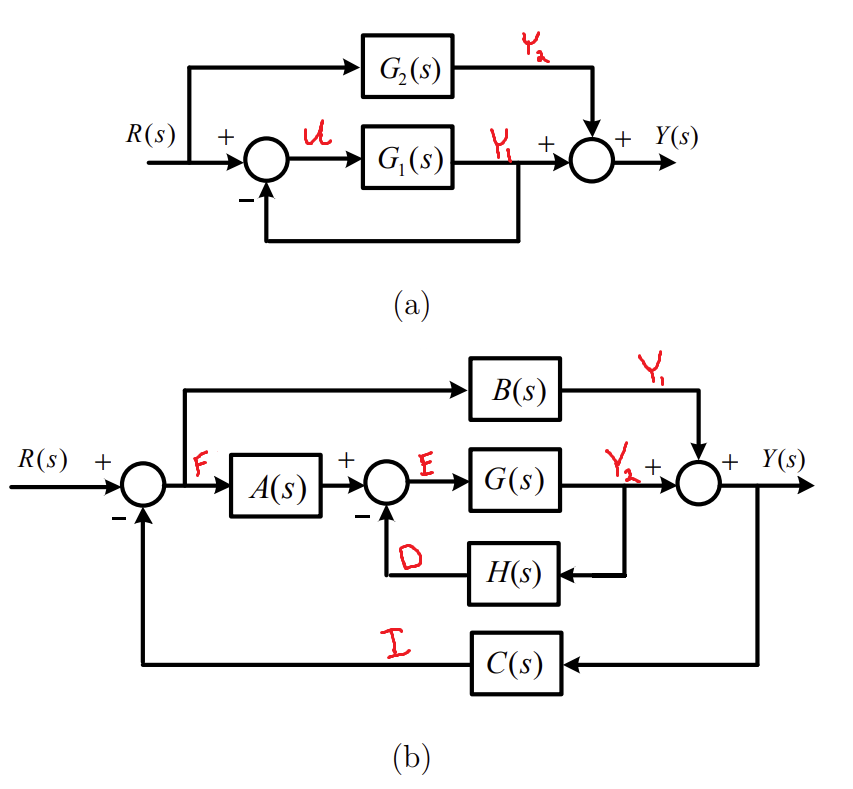
\includegraphics[width=0.55 \linewidth]{prob1}
    \caption{Problem 1}
    \label{fig:p1}
\end{figure}

\soln

\begin{enumerate}[a)]
    \item $Y(s) = Y_1(s) + Y_2(s) = G_1(s) U(s) + G_2(s)R(s)$,\\
    $U(s) = R(s) - G_1(s)U(s) \implies (1 + G_1(s))U(s) = R(s) \implies U(s) = \frac{R(s)}{1 + G_1(s)}$ \\
    So, $Y(s) = \left[\frac{G_1(s)}{1 + G_1(s)} + G_2(s)\right] R(s)$
\end{enumerate}



\problem{2}
Determine the time constant of the system:
\begin{figure}[h] 
    \centering
    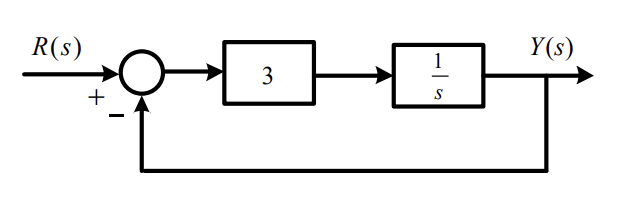
\includegraphics[width=0.55 \linewidth]{prob2}
    \caption{Problem 2}
    \label{fig:p2}
\end{figure}

\soln




\problem{3}
Specify the gain K
of the proportional controller so that the output $y(t)$ has an overshoot of no more then 10\%
in response to a unit step

\begin{figure}[h] 
    \centering
    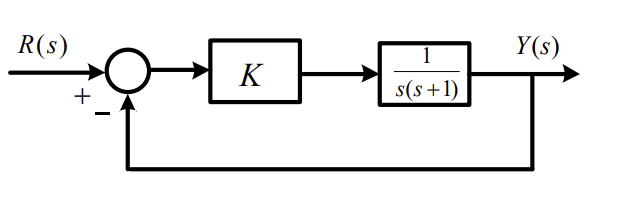
\includegraphics[width=0.55 \linewidth]{prob3}
    \caption{Problem 3}
    \label{fig:p3}
\end{figure}

\soln








\problem{4}

Consider the system
\begin{figure}[h] 
    \centering
    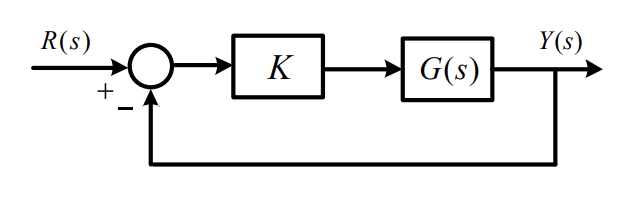
\includegraphics[width=0.55 \linewidth]{prob4}
    \caption{Problem 4}
    \label{fig:p4}
\end{figure}

with \begin{enumerate}[a)]
    \item $KG(s) = \frac{4(s+2)}{s(s^3+2s^2+3s+4)}$
    \item $KG(s) = \frac{2(s+4)}{s^2(s+1)}$
\end{enumerate}

Use Routh's stability criterion to determine whether the each of the resulting closed-loop
system will be asymptotically stable.

\soln







\problem{5}
Using Routh's stability criterion to determine how many roots with positive
real parts the following equations have: 

\begin{enumerate}[a)]
    \item $s^4 + 8s^3 + 32s^2 + 80s + 100 = 0$
    \item $s^5 + 10s^4 + 30s^3 + 80s^2 + 344s + 480 = 0$
\end{enumerate}

\soln





\problem{6}

Consider the closed-loop system:
\begin{figure}[h] 
    \centering
    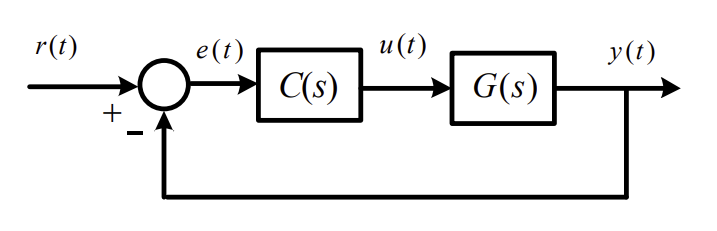
\includegraphics[width=0.55 \linewidth]{prob6}
    \caption{Problem 6}
    \label{fig:p6}
\end{figure}

$G(s) = \frac{1}{s^2}$, and $C(s) = \frac{10(s+2)}{s+5}$.

Find the system type and determine the steady state tracking errors for:

\begin{enumerate}[a)]
    \item $r(t) = 1(t)$
    \item $r(t) = t1(t)$
    \item $r(t) = 1/2 t^2 1(t)$
\end{enumerate}

\soln




\problem{7}
Sketch the Nyquist plot for an open-loop system with transfer function:
\begin{enumerate}[a)]
    \item $G(s) = \frac{1}{s^2}$
    \item $G(s) = \frac{1}{s^2 + 4}$
\end{enumerate}

\soln







\problem{8}
Consider the system with loop gain
$$
L(s) = KG(s) = \frac{K(s+2)}{s+10}
$$
Use Matlab command nyquist to plot nyquist plot for $G(s)$, and based
on the nyquist plot, determine the range of $K$ for which the closed-loop system is asymptotically stable
\soln




\problem{9}
Is the following system controllable? Observable?

\begin{align*}
    \dot{x} &= \begin{bmatrix}
        0 & 1 \\ -1 & -1
    \end{bmatrix} x + \begin{pmatrix}
        0 \\ 1
    \end{pmatrix} u \\
    y &= \begin{pmatrix}
        1 & 0
    \end{pmatrix} x
\end{align*}

\soln



\end{document}